\section{Implementation aspects}
\label{cap:Implementation}

Following section shows how the theoretical concept of Kalman filter and MPC (see sections \ref{cap:kalman_filter_theory} and \ref{cap:mpc_theory}) was transferred to the real hardware. Although its implementation may seem easy and it is simple and straightforward when using e.g. Matlab, the transfer of the technology into embedded hardware brings in new challenges. We propose practical refinements that allow execution of MPC on underpowered hardware of the UAV. We present an approach how to exploit the structure of the dynamical system to introduce off-set free tracking with the original MPC formulation. Subsequently, we discuss how to take an advantage of the objective's structure to optimized it while having a small memory footprint. Lastly, parameters of MPC are tuned to meet the performance requirements (namely computation rate). Furthermore, the simulation results are presented to allow comparison with experiments.

The final setup comprises of two separate MPC controllers driving both attitude axis. Since the PID altitude controller developed during previous work \citep{endrych2014} is satisfactory for experiments with multiple UAVs, implementation of the MPC for the altitude system was postponed for future work. Because both attitude axis are controlled identically (due to decoupled system description), following chapters contain figures mostly of forward motion of the UAV. The yaw subsystem is left uncontrolled due to absence of data for estimating angle $\phi$ but considering its stability and the order of the dynamical system, appropriate PD controller could be designed to suite our needs.

\subsection{Implementing Kalman filter}

The KF, as it is described in section \ref{cap:kalman_filter_theory}, was firstly simulated in Matlab. In order to provide good estimate all states, one has to identify the measurement noise $\textbf{Q}$ and tune the process noise parameters in \textbf{R}. Practically, setting of kalman filter is done by tuning the ratio between elements of $\textbf{R}$ and $\textbf{Q}$. For the system defined by (\ref{eq:attitude_LTI}) these were stated as follow

\begin{equation}
\textbf{R}_{x,y} = \begin{bmatrix}
1 & 0 & 0 \\
0 & 1 & 0 \\
0 & 0 & 1 \\
\end{bmatrix}, 
\textbf{Q}_{x, y} = \begin{bmatrix}
150
\end{bmatrix}
\label{eq:kf_RQ_simple}
\end{equation}

The remaining parameters for KF are $\textbf{C}_{x, y} = \left[0, 1, 0\right]$ and LTI system matrices defined as (\ref{eq:attitude_LTI_identified}). Tuning the filter is a very subjective process where one has to take into account several criteria, often contradictory. One needs to estimate all states as accurate as possible while having them converge as fast as possible (increasing values of \textbf{R}). On the other hand, it is supposed to eliminate the measurement noise (increasing values of \textbf{Q}) which brings a possibility of an incorrect estimate. The rule of thumb is to give a priority to convergence by finding a noise level which is the highest tolerable to allow smooth control. The corresponding ratio (\ref{eq:kf_RQ_simple}) was found roughly in simulation and lately fine-tuned on hardware.

The filter was firstly implemented solely on the xMega MCU. Because the MCU allowed its execution only in a rate around $50\jed{Hz}$ while dedicating all its resources, it was moved on the STM MCU. There the computation is done under $1\jed{ms}$ for both axis.

\subsubsection{Estimating state disturbances}

The Kalman filter can be also used for estimation of disturbances, when one is able to model them as a state in the LTI system. In our case, these are uncontrollable and unmeasurable states, that have a link into the path between the system input and a measured state. Specifically, all disturbances in the system of the UAV can be combined into one force acting on its body. In practice, these are for example the wind disturbances and IMU calibration offset. The force can be expressed as an \textit{parasitic} acceleration in the respective attitude axis. 

Let us improve the attitude LTI system by adding two new states --- $x_d$ representing the disturbance in acceleration and $x_2$ representing the sum of the disturbance and the state $x_1$ that was previously considered as the acceleration. Figure \ref{fig:LTI_with_disturbances} shows the diagram of the newly proposed system 

\begin{figure}[h]	
\centering
\begin{tikzpicture}[->,>=stealth',node distance=1.5cm]

	\node[nothing] (vstup) {
 	};
 	
	\node[state, right of = vstup, shift = (right:0.5cm)] (kk2) {
  		$\frac{1}{\tau_1s + 1}$
 	};
 	
 	\node[input, right of = kk2, shift = (right:0.5cm), shift = (down:0.7cm) ] (adder) {
		+
 	};
 	
 	\node[nothing, below of = kk2, shift = (right:0.3cm)] (disturbance) {
		$\ddot{x}_d(s)$
 	};
 	
	\node[state, right of = adder, shift = (right:0.5cm)] (int1) {
  		$\frac{1}{s}$
 	};
 	
	\node[state, right of = int1, shift = (right:0.5cm)] (int2) {
  		\large{$\frac{1}{s}$}
 	};
 	
	\node[nothing, right of = int2, shift = (right:0.2cm)] (output) {
 	};

	\path (vstup.east)+(0.7cm, 0.3cm) node (label0) {\textbf{$u(s)$}};
	\path (kk2.east)+(0.8cm, 0.3cm) node (label1) {\textbf{$\ddot{x}_u(s)$}};
	\path (adder.east)+(0.7cm, 0.3cm) node (label2) {\textbf{$\ddot{x}(s)$}};
	\path (int1.east)+(0.7cm, 0.3cm) node (label3) {\textbf{$\dot{x}(s)$}};
	\path (int2.east)+(0.7cm, 0.3cm) node (label4) {\textbf{$x(s)$}};
       
	\path[->] (vstup) edge ($(kk2.west)$);
	\path[->] ($(kk2.east)$) edge [bend left=15] (adder);
	\path[->] (disturbance) edge [bend right=15] (adder);
	\path[->] (adder) edge ($(int1.west)$);
	\path[->] (int1.east) edge ($(int2.west)$);
	\path[->] (int2.east) edge (output);

\end{tikzpicture}
\caption{Diagram of the LTI system with the disturbance estimation.}
\label{fig:LTI_with_disturbances}
\end{figure}

where $u(s)$ is the Laplace image of the input signal $u(t)$, and $x(s)$, $\dot{x}(s)$, $\ddot{x}(s)$, $\ddot{x}_u(s)$, $\ddot{x}_d(s)$ are Laplace images of $x(t)$, $\dot{x}(t)$, $\ddot{x}(t)$, $\ddot{x}_u(t)$, $\ddot{x}_d(t)$ respectively. Furthermore, the disturbance can be estimated by the KF by carefully setting the process noise matrix $\textbf{R}$. If we set relatively high variances for states $\ddot{x}_u$, $\ddot{x}$ compared to state $\ddot{x}_d$ the filter will estimate $\ddot{x}_d$ by computing discrepancies between estimations from $u$ and corrections from measured $\dot{x}$.

Matrices for the new discrete attitude LTI system states as follows	

\begin{equation}
\begin{split}
\mathbf{A}_{x, y} = \begin{bmatrix}
1 & 0.0114 & 0 & 0 & 0 \\
0 & 1 & 0.0114 & 0 & 0\\
0 & 0 & 0 & 1 & 1 \\
0 & 0 & 0 & 0.9799 & 0 \\
0 & 0 & 0 & 0 & 1
\end{bmatrix}, \mathbf{B}_{x, y} = \begin{bmatrix}
0\\
0\\
0\\
5.0719 \times 10^{-5}\\
0
\end{bmatrix}
\end{split}
\label{eq:attitude_LTI_big_identified}
\end{equation}

where the state vectors are $\mathbf{q}_{x} = \left(x, \dot{x}, \ddot{x}, \ddot{x}_u, \ddot{x}_d\right)^T$ and $\mathbf{q}_{y} = \left(y, \dot{y}, \ddot{y}, \ddot{y}_u, \ddot{y}_d\right)^T$ respectively. This state representation was used in the final implementation and during experiments. One can effectively tune the parameters of KF that the settling time is fast enough to compensate for wind disturbances. The diagonal of the process noise matrix was set to $\mathrm{diag}(\textbf{R})~=~\left(1, 1, 1, 1, 0.04\right)^T$ in the final implementation. Estimated disturbances can be further used in the control loop to eliminate control offset (see section \ref{cap:offset_free_tracking}). It can be also used for detecting abnormal flight conditions as a part of a failure detection system.
 
\subsection{Implementing QMPC}
\label{cap:implementing_qmpc}

There are two points of view on model predictive control. It can be either used for trajectory planning or for real-time control solely. Given the dynamical model, set of constraints and roughly defined (even infesible) desired trajectory, it can produce a feasible one (satisfying constraints and the dynamical model) when minimizing a certain objective. In this form, it can be used as an offline trajectory planner \citep{saska2014formations}. On the other hand, when using the MPC for real-time control of the UAV, we suppose that the desired trajectory is already known and that it is feasible. It has a significant impact on the particular formulation of our MPC. If the trajectory is feasible (meaning no state constraints are violated) and it initiates in the current state of the UAV, there will be no state constraints violated (and thus required) in the MPC formulation, otherwise the trajectory is not feasible. Based on these assumptions we propose an implementation of \emph{input constrained QMPC}. Since the feasibility of the desired trajectory may not be guaranteed or the trajectory may not start with the current state of the UAV, we propose a simple \emph{input governor} (see section \ref{cap:input_governor}) which is a recommended technique \citep{rossiter2013mpcpracticalapproach} in place of implementing constraints.

Since optimizing the objective, constrained only by input constraints is substantially easier than solving the state-constrained MPC, we can afford to optimize over a larger prediction horizon. It allows the UAV to track dynamic trajectories with greater precision since the controller can be more proactive with regards to future changes in the desired trajectory.  


\subsubsection{Input governor}
\label{cap:input_governor}

In order to provide a trajectory tracking that does not violate state constraints, there are two situations that should be watched over. Firstly, the trajectory itself should satisfy the system dynamics and imposed constraints and secondly the trajectory should start with the current state of the UAV. The \emph{input governor} is a system that modifies the desired trajectory in such a way, that it satisfies these requirements. The modification does not necessary need to be optimal since our aim is not to produce optimal desired trajectories but to find optimal control actions to drive the system through known trajectories. The governor produces a feasible trajectory from the current state of the UAV. The only constraint we impose is a maximum speed of the UAV--- the \emph{px4flow} sensor effectively measures speed only up to $0.35\jed{ms^{-1}}$. Our input governor limits the rate of change of the desired position trajectory by that value while ensuring the trajectory initiates in the current state of the UAV.

\subsubsection{Offset-free tracking}
\label{cap:offset_free_tracking}

The MPC formulation as stated in section \ref{cap:mpc_formulation} does not necessary provide offset-free tracking. In the case of external disturbances or imperfect behavior of the integrated stabilization system, this would lead to steady state control error. There are several techniques to solve the problem, the classical one is a \emph{delta input formulation of MPC} \citep{borrelli2007offsetfree}. One could even create an additional integral feedback loop around the MPC controller. But since our estimator is able to observe the disturbance within the system, the classical formulation of MPC is in fact able to control the system without a steady state error \citep{rossiter2013mpcpracticalapproach}. Moreover it has some other useful properties --- there are no windup issues (like with classical integral feedback) and the controller (considering its separation from the estimator) can be completely stateless. 

With this approach, the controller is able to compensate not only for small and steady disturbances, but it creates adequate actions even for sudden and momentary disturbances. See section \ref{cap:momentary_disturbances} for results of the experiments.

\subsubsection{Controller parameters}
\label{cap:implementation_performance}

There are several parameters whose settings have an impact on performance of the controller. Some of them are tied up by execution rate of the MPC, namely the number of decision variables and the length of the prediction horizon.  After a testing, we have converged to horizon length of 200 steps ($2.2\jed{s}$) with 20 decision variables in the objective. They are distributed in an exponential way over the horizon. First 10 variables directly correspond to first 10 control actions. Another 9 variables cover control actions evenly up to the 100th one. The last variable sets the control action for the last 100 steps.

Our system presumes desired trajectories in the form of position states only. There is no need to require the information about the desired velocity of the UAV, unless its speed is the only state that should be controlled without demanding the control of UAV's position. One can specify not to penalize certain states by setting respective elements of matrices $\textbf{Q}$, $\textbf{S}$ and $\textbf{P}$ (consequently merged to \textbf{\^Q}, \textbf{\^P}) to zero. By doing that, the control error of the state does not take part in the objective. This leaves us basically three parameters to set in order to tune the performance of the controller, supposing the desired trajectory consists of only position state. These parameters are weights for penalizing position errors and control actions as defined in section \ref{cap:mpc_formulation}, specifically tuned as follows

\begin{table}
\centering
\begin{tabular}{ll}
\hline
Horizon length & 200 steps, $2.2\jed{s}$ \\
Number of variables & 20 \\
Move blocking & exponential-like \\
Constraints & input constraints \\
MPC rate & 30\jed{Hz} \\
\hline
\end{tabular}
\caption{Parameters of our MPC implementation.}
\label{tab:mpc_parameters}
\end{table}


\begin{equation}
\textbf{Q} = \begin{bmatrix}
1.07 & 0 & 0 & 0 & 0 \\
0 & 0 & 0 & 0 & 0 \\
0 & 0 & 0 & 0 & 0 \\
0 & 0 & 0 & 0 & 0 \\
0 & 0 & 0 & 0 & 0
\end{bmatrix}, \textbf{S} = \begin{bmatrix}
10 & 0 & 0 & 0 & 0 \\
0 & 0 & 0 & 0 & 0 \\
0 & 0 & 0 & 0 & 0 \\
0 & 0 & 0 & 0 & 0 \\
0 & 0 & 0 & 0 & 0
\end{bmatrix}, \textbf{P} = \begin{bmatrix}
0.0000025
\end{bmatrix}
\label{eq:QSP_matrices}
\end{equation}

Tuning of MPC controller is a different process than tuning of e.g. PID controller. Its parameters (diagonals of matrices in (\ref{eq:QSP_matrices})) have a meaningful interpretation --- they correspond to a particular state and the effect of changing them can be observed on them. A common rule of thumb is to firstly normalize the diagonal of \textbf{Q} according to a \textit{'usual'} range of state's values (e.g. if the range of the velocity state is $0.1\jed{ms^{-1}}$ then the corresponding element of \textbf{Q} is set to $1/0.1$). For the start, this helps to normalize the penalties, since each state can hypothetically have a different unit of measurement and the typical range of values. Furthermore the parameter \textbf{P} can be set so the system produces adequate control actions --- such that does not violate input constraints when started from an ordinary initial condition. On can set \textbf{P} in such a way that actions produced lie within a desired range, most of the time. When increasing the input penalization, generated control actions tend to be smaller --- the system is more conservative with actions. Finally one can tune elements \textbf{Q} so the states change as wanted.

There is important a phenomenon that needs to be taken into account. The matrix \textbf{\^H} (defined in (\ref{eq:mpc_objective_large})) determines the shape of the quadratic form in the objective. A condition number of \textbf{\^H} determines whether the optimum of the objective is sharply defined or whether it lies within a wide plateau. See figure \ref{fig:quad_form_conditionality} for an illustrative example on 2-dimensional quadratic form. In the case of ill-conditioned quadratic form, there are many solutions with the objective value near the optimum --- this can be interpreted as there are many different sequences of control actions, that can lead to similar outcomes. We should avoid constructing such function, because locating its minimum may lead to numerical difficulties during calculations. Optimizing it using a closed-form as described in section \ref{cap:qmpc_unconstrained} can be affected by numerical instabilities when calculating the matrix inversion $\textbf{\^H}^{-1}$. Also, iterative methods tend to suffer from slow convergence on such plateaus \citep{boyd2004convex}. Fortunately, it has a simple solution. We can regularize the matrix \textbf{\^H} by increasing penalization \textbf{\^P} since it directly increases values on its diagonal and thus increases its eigenvalues (supposing $\textbf{\^P} \succ 0$). The interpretation is simple --- we limit the freedom of input actions by regularizing \textbf{\^H} which leads to better numerical stability of computation.

\begin{figure}
\centering

\begin{subfigure}[b]{0.5\textwidth}
	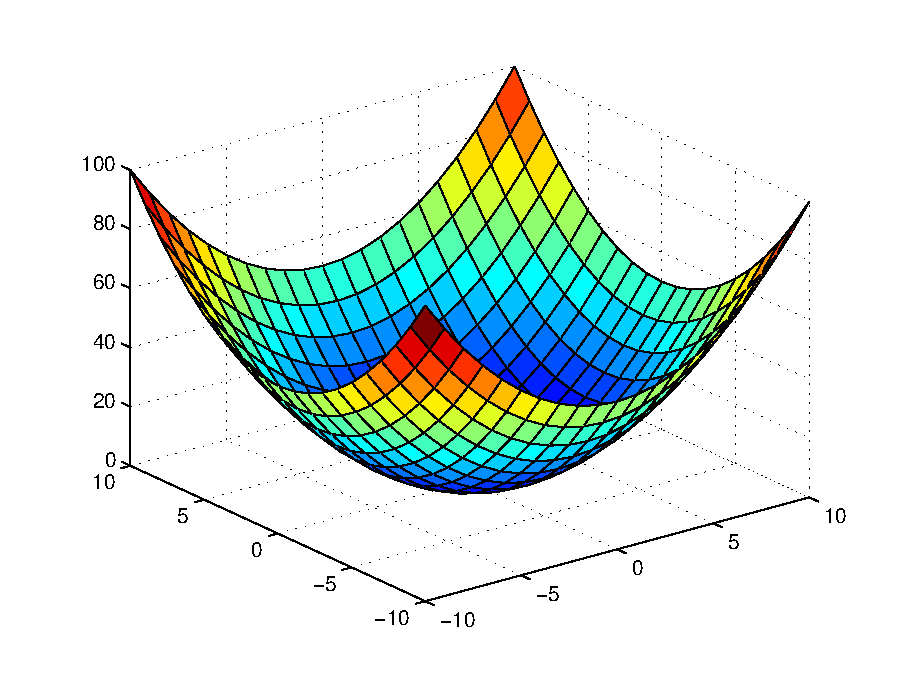
\includegraphics[width=\textwidth]{fig/quadform1.eps}
	\caption{well-conditioned quadratic form}
	\label{fig:quad_form_well_conditioned}
\end{subfigure}%
\begin{subfigure}[b]{0.5\textwidth}
	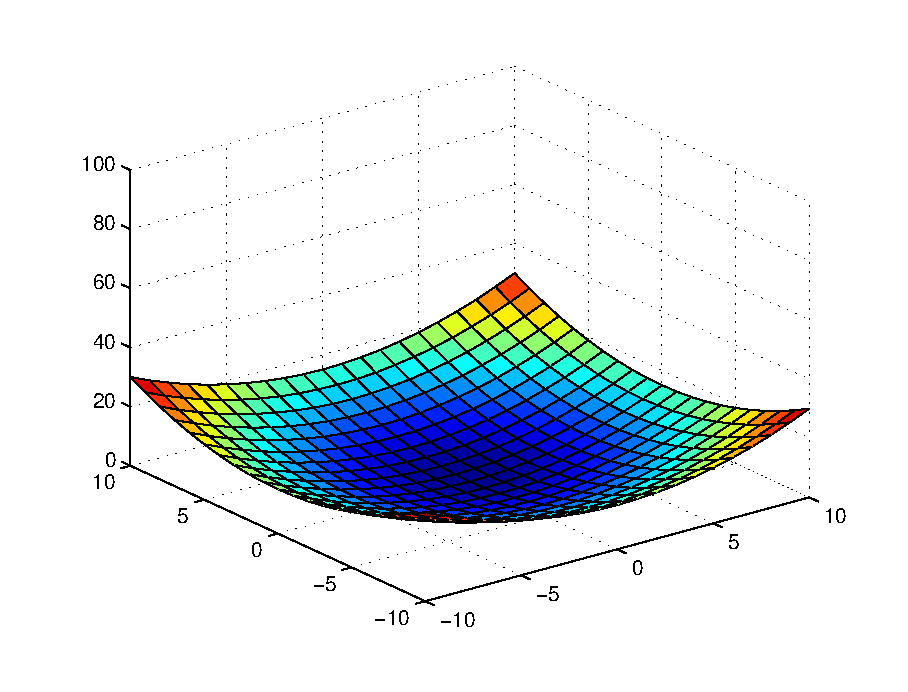
\includegraphics[width=\textwidth]{fig/quadform2.eps}
	\caption{ill-conditioned quadratic form}
	\label{fig:quad_form_ill_conditioned}
\end{subfigure}

\caption{Illustrative example of 2-dimensional quadratic form.}
\label{fig:quad_form_conditionality}
\end{figure}

\subsubsection{Optimizing onboard}

When implementing the \emph{input constrained MPC} into embedded hardware, the structure of the problem can be exploited in following way. Since matrix \textbf{\^H} does not depend on the desired trajectory nor the initial condition, it can be precomputed offline. This also holds for its inversion $\textbf{\^H}^{-1}$ and matrices \textbf{\^B} and \textbf{\^A}. Thanks to that we can store them in a ROM (read-only memory, designated for the program) which supports execution even on a microcontrollers with a small amount of RAM.

The workflow of testing and tuning different parameters of the controller was built upon a simulation in Matlab. One part of its parts is a script that can generate a \verb!C! code, with all matrices precomputed, that can be easily inserted into sources for the STM microcontroller. This allowed relatively easy tuning and testing cycle.

\subsection{Summary}

Previous chapter described some aspects of the implementation of Kalman filter and MPC controller. Particular settings of Kalman filter are presented followed by the extension of the LTI system to allow estimating state disturbances. Then we discussed the two fundamental approaches to use MPC --- as a trajectory planner and as a low-level controller. The input governor system is presented to supply the controller with a feasible trajectory followed by particular settings of our MPC implementation. Finally we discussed a memory allocation of MCP matrices need for final implementation.